 
%______________________________________________________________________________________________________________________
% @brief    LaTeX2e Resume for Kamil K Wojcicki
\documentclass[margin,line]{resume}
\usepackage[latin1]{inputenc}
\usepackage{graphics}
\usepackage{amsmath,amssymb}
\usepackage{gensymb}
\usepackage{amsthm}
\usepackage{wrapfig,lipsum,booktabs}
\usepackage{caption}
\usepackage{subcaption}
\usepackage{tabulary}
\usepackage{epigraph}
\usepackage{mwe}
\usepackage[autostyle]{csquotes} 
\usepackage{lipsum,lmodern}
\usepackage[skins]{tcolorbox}
\usepackage{pgf,tikz}
\usetikzlibrary{arrows,shapes,backgrounds,fit}
\usetikzlibrary{arrows,automata}

\usepackage{fancyvrb}
\usepackage{listings}
\usepackage{color}
%______________________________________________________________________________________________________________________
\begin{document}
\name{\Large Simon Holmbacka. PhD -- 10 Most important publications}
\begin{resume}
\begin{picture}(320,0)
\put(320,-160){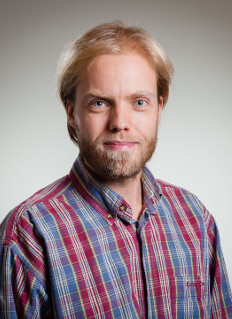
\includegraphics[scale=0.5]{simon.jpg}}
\end{picture}
    %__________________________________________________________________________________________________________________
    % Contact Information
    \section{\mysidestyle Contact\\Information}

    Embedded Systems Laboratory                         	     \vspace{0mm}\\\vspace{0mm}%
    Faculty of Science and Engineering                           \vspace{0mm}\\\vspace{0mm}%
    \AA{}bo Akademi University, Finland			       		\vspace{0mm}\\\vspace{-4.5mm}%
    
\small{
    Tammikalliontie 1			\vspace{0mm}\\\vspace{0mm}%
    20900				\vspace{0mm}\\\vspace{0mm}%
    Turku				\vspace{0mm}\\\vspace{0mm}%
    Finland				\vspace{0mm}\\\vspace{0mm}%
    Tel: +358 50 5310467		\vspace{0mm}\\\vspace{0mm}%
    Email: sholmbac@abo.fi		\vspace{0mm}\\\vspace{-4.5mm}%
    }
\vspace{1.0cm}
\section{\mysidestyle Thesis}    
Simon Holmbacka:
\textit{Energy Aware Software for Many-Core Systems},
Faculty of Science and Engineering,\\ \AA{}bo Akademi University, 2015, Turku, Finland

Simon Holmbacka, J\"{o}rg Keller
\textit{Workload Type-Aware Scheduling on big.LITTLE Platforms}
\textsl{Proceedings of the 17th International Conference on Algorithms and Architectures on Parallel Processing}, 2017, Helsinki, Finland

Simon Holmbacka, Dra\v{z}en Lu\v{c}anin , Ilia Pietri, Ivona Brandic, Johan Lilius, Rizos Sakellariou:
\textit{Performance-Based Pricing in Multi-Core Geo-Distributed Cloud Computing}, 
\textsl{IEEE Transactions on Cloud Computing}, IEEE 2016

Simon Holmbacka, J\"{o}rg Keller, Patrick Eitschberger, Johan Lilius:
\textit{Accurate Energy Modeling for Many-Core Static Schedules with Streaming Applications}, 
\textsl{Microprocessors and Microsystems, Elsevier}, 2016

Simon Holmbacka, Erwan Nogues, Maxime Pelcat, S\'{e}bastien Lafond, Daniel Menard, Johan Lilius:
\textit{Energy-Awareness and Performance Management with Parallel Dataflow Applications}, 
\textsl{The Journal Signal Processing Systems. Springer US}, 2015

Simon Holmbacka, J\"{o}rg Keller
\textit{Workload Type-Aware Scheduling on big.LITTLE Platforms}
\textsl{Proceedings of the 17th International Conference on Algorithms and Architectures on Parallel Processing}, 2017, Helsinki, Finland

Simon Holmbacka, Robert M\"{u}ller: 
\textit{epEBench: True Energy Benchmark},
\textsl{25st Euromicro International Conference on Parallel, Distributed and Network-Based Processing}, 2016, St Petersburg, Russia

Simon Holmbacka, S\'{e}bastien Lafond, Johan Lilius:
\textit{Performance Monitor Based Power Management for big.LITTLE Platforms}
\textsl{HiPEAC Workshop on Energy Efficiency with Heterogeneous Computing}, 2015, Amsterdam, Netherlands

Simon Holmbacka, Erwan Nogues, Maxime Pelcat, S\'{e}bastien Lafond, Johan Lilius:
\textit{Energy Efficiency and Performance Management of Parallel Dataflow Applications} [\textbf{BEST PAPER}]
\textsl{The 2014 Conference on Design \& Architectures for Signal \& Image Processing}, 2014, Madrid, Spain

Simon Holmbacka Fredric H\"{a}llis, Wictor Lund, S\'{e}bastien Lafond and Johan Lilius:
\textit{Energy and Power Management, Measurement and Analysis for Multi-Core Processors} 
\textsl{TUCS Technical Reports 1117}, 2014, Turku Centre for Computer Science 




%______________________________________________________________________________________________________________________

\include{ecourse}

\end{resume}
\end{document}


%______________________________________________________________________________________________________________________
% EOF

